%%%%%%%%%%%%%%%%%%%%%%%%%%%%%%%%%%%%%%%%%%%%%%%%%%%%%%%%%%%
% --------------------------------------------------------
%  ____  _           
% |  _ \| |__   ___  
% | |_) | '_ \ / _ \ 
% |  _ <| | | | (_) |
% |_| \_\_| |_|\___/ 
%
% LaTeX2e Template
% Version 3.0.0 (24/02/2026)
%
% Author: 
% Guillermo Jimenez (memo.notess1@gmail.com)
% 
% Contributor:
% Eduardo Gracidas (eduardo.gracidas29@gmail.com)
%
% License:
% Creative Commons CC BY 4.0
% --------------------------------------------------------
%%%%%%%%%%%%%%%%%%%%%%%%%%%%%%%%%%%%%%%%%%%%%%%%%%%%%%%%%%%
% --------------------------------------------------------
% Find the latest version on GitHub:
% https://github.com/MemoJimenez/Rho-class
% --------------------------------------------------------
%%%%%%%%%%%%%%%%%%%%%%%%%%%%%%%%%%%%%%%%%%%%%%%%%%%%%%%%%%%

\documentclass[9pt,a4paper,oneside]{rho-class/rho}
\usepackage[spanish,es-nodecimaldot,es-noindentfirst]{babel}

%% Spanish babel recomendation
% \usepackage[spanish,es-nodecimaldot,es-noindentfirst]{babel}

%----------------------------------------------------------
% Title
%----------------------------------------------------------

\doctype{Documentation Template}
\title{Parcial 1 señales y sistemas 2: Demodulador FSK para el estándar P25}

%----------------------------------------------------------
% Authors, Affiliations and dates
%----------------------------------------------------------

\author[a,1]{Juan Felipe Calixto Londoño}
\author[a,2]{José Luis Gómez Sierra}
\author[a,3]{Juan Manuel Sarmiento Parra}

%----------------------------------------------------------

\affil[a]{Universidad Nacional de Colombia, Facultad de Ingeniería}

%----------------------------------------------------------

\dates{Semestre 2026-1}

%----------------------------------------------------------
% Corresponding author-, Document- information
%----------------------------------------------------------

\corres{\textsuperscript{\textasteriskcentered}Autores correspondientes: 
\href{mailto:jcalixtol@unal.edu.co}{jcalixtol@unal.edu.co}
\href{mailto:jogomezsi@unal.edu.co}{jogomezsi@unal.edu.co}
\href{mailto:jusarmientop@unal.edu.co}{jusarmientop@unal.edu.co}}


\journalname{LATEX}
\journal{Rho-class (v.3) 2026}
\theday{\today}
\vol{X}
\no{X}

%----------------------------------------------------------
% Abstract and Keywords
%----------------------------------------------------------

\begin{abstract}
    Este informe es realizado con el fin de explicar exhaustivamente la realización del primer parcial de la asignatura, de forma que se entienda cuales fueron los cálculos realizados y sus respectivas fórmulas utilizadas, el "porqué" se realiza la elección de ciertos filtros por encima de otros, y de intentar entender a cabalidad la realización de estos en MatLab.
\end{abstract}

%----------------------------------------------------------

\keywords{Filtros analógicos, Filtros Digitales, MatLab, Señales}

%----------------------------------------------------------

\begin{document}

    \maketitle
    \thispagestyle{firststyle}

%----------------------------------------------------------

\section{Punto 1: Análisis Teórico y Códigos de MATLAB}

    En este punto del taller se analizaron los requerimientos teóricos necesarios para el diseño del demodulador FSK según el estándar P25. El sistema utiliza modulación 4-FSK (Frequency Shift Keying de 4 niveles), donde la información se codifica en cuatro frecuencias distintas para la portadora. Según el estándar, estas frecuencias centrales están definidas como:
    \begin{itemize}
        \item Símbolo '+3': $f_1 = 10700$ Hz
        \item Símbolo '+1': $f_2 = 11900$ Hz
        \item Símbolo '-1': $f_3 = 13100$ Hz
        \item Símbolo '-3': $f_4 = 14300$ Hz
    \end{itemize}
    La separación entre cada frecuencia adyacente es estricta, limitándose a apenas $1200$ Hz. Esto impone un reto de diseño crítico, requiriendo filtros con bandas de transición sumamente angostas y alta ortogonalidad para mitigar agresivamente el ruido de banda adyacente e impedir la diafonía o interferencia entre símbolos (ISI). Para cumplir con estas demandas topológicas y aislar el símbolo adecuado con alta pureza espectral, se sintetizan en paralelo cuatro filtros selectivos: un filtro pasabajos (dedicado a retener unicamente $f_1$), un par de filtros pasabandas de alta Q (para capturar por separado $f_2$ y $f_3$), y finalmente un filtro pasaaltos (asignado al canal $f_4$). Las frecuencias perimetrales de corte se proyectan sobre los ejes intermedios de los lóbulos de portadora (aproximadamente en $11300$ Hz, $12500$ Hz y $13700$ Hz), logrando rechazar de forma tajante el contenido espurio fuera del intervalo de interés.

    \subsection{Implementación matemática y diseño en MATLAB}

    Para la comprobación y el modelado matemático del banco de filtros, el código en MATLAB define inicialmente las atenuaciones objetivo en las bandas pasa y de rechazo (\texttt{Rp = 1} dB, y \texttt{Rs = 15} dB). Adicionalmente, se obtienen las características de la señal a analizar:

\begin{minted}[linenos,fontsize=\small]{matlab}
Rp = 1;
Rs = 15;

Fs = 75000;
t = (0:length(Out)-1)/Fs;

N = length(Out);
f = (0:N-1)*Fs/N;
X = fft(Out);
\end{minted}

    Posteriormente, debido a que la modulación puede poseer un ensanchamiento frecuencial pequeño, se establece un margen para las frecuencias de corte, utilizando:
    
    \begin{itemize}
        \item \textbf{Filtro Pasabajos:} Diseñado con $f_p = 10.31$ kHz y $f_s = 11.56$ kHz. Su diseño se centró en retener la polaridad del símbolo $+3$.
        \item \textbf{Filtros Pasabanda 1 y 2:} Diseñados estableciendo rangos de paso entre $10.92$ kHz $\approx 12.46$ kHz; y el segundo entre $12.46$ kHz $\approx 14.05$ kHz (ajustando para garantizar mínimas interferencias interbanda según el script).
        \item \textbf{Filtro Pasaaltos:} Frecuencia de transición a partir del corte ideal $13.43$ kHz y banda de paso plenamente establecida en $14.68$ kHz para extraer el símbolo $-3$.
    \end{itemize}

    Se usa la función \texttt{cheb1ord} de la señal para calcular el orden prototipo analógico indispensable en todos los filtros, forzando un $N_{max}$ aplicable a todos de igual manera para uniformidad del sistema. Luego de obtener los coeficientes en el dominio de la variable $s$ usando la instrucción \texttt{cheby1(n, Rp, Wn, ... , 's')}:

\begin{minted}[linenos,fontsize=\small]{matlab}
nPB = max(n2,n3); % mismo orden para pasabanda
nEXT = max(n1,n4); % mismo orden para extremos

[b1,a1] = cheby1(nEXT,Rp,Wn1,'low','s');
[b2,a2] = cheby1(nPB,Rp,Wn2,'bandpass','s');
[b3,a3] = cheby1(nPB,Rp,Wn3,'bandpass','s');
[b4,a4] = cheby1(nEXT,Rp,Wn4,'high','s');
\end{minted}

    Observamos individualmente las respuestas en frecuencia que confirman que la caída por década es lo bastante pronunciada:

    \begin{figure}[H]
        \centering
        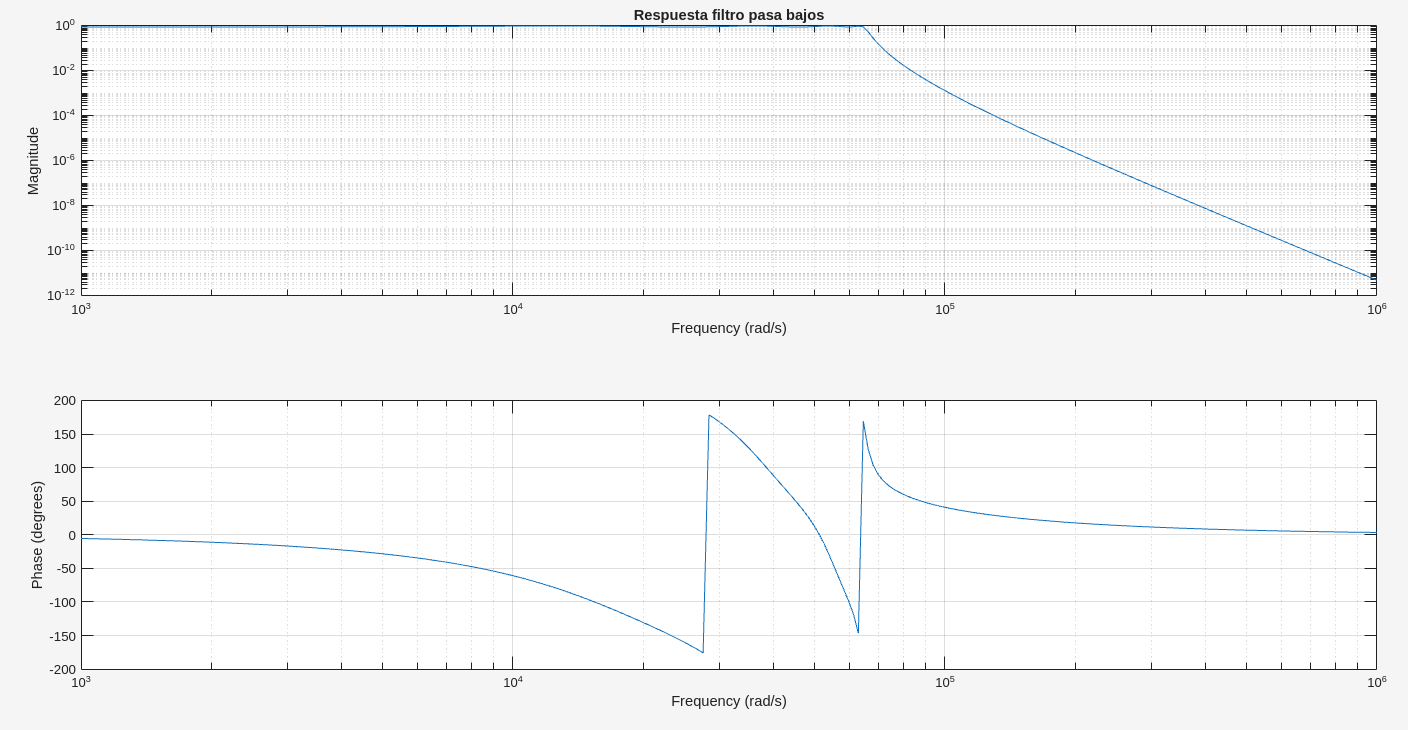
\includegraphics[width=0.42\columnwidth]{figures/Punto1/pasabajos_analogico.png}
        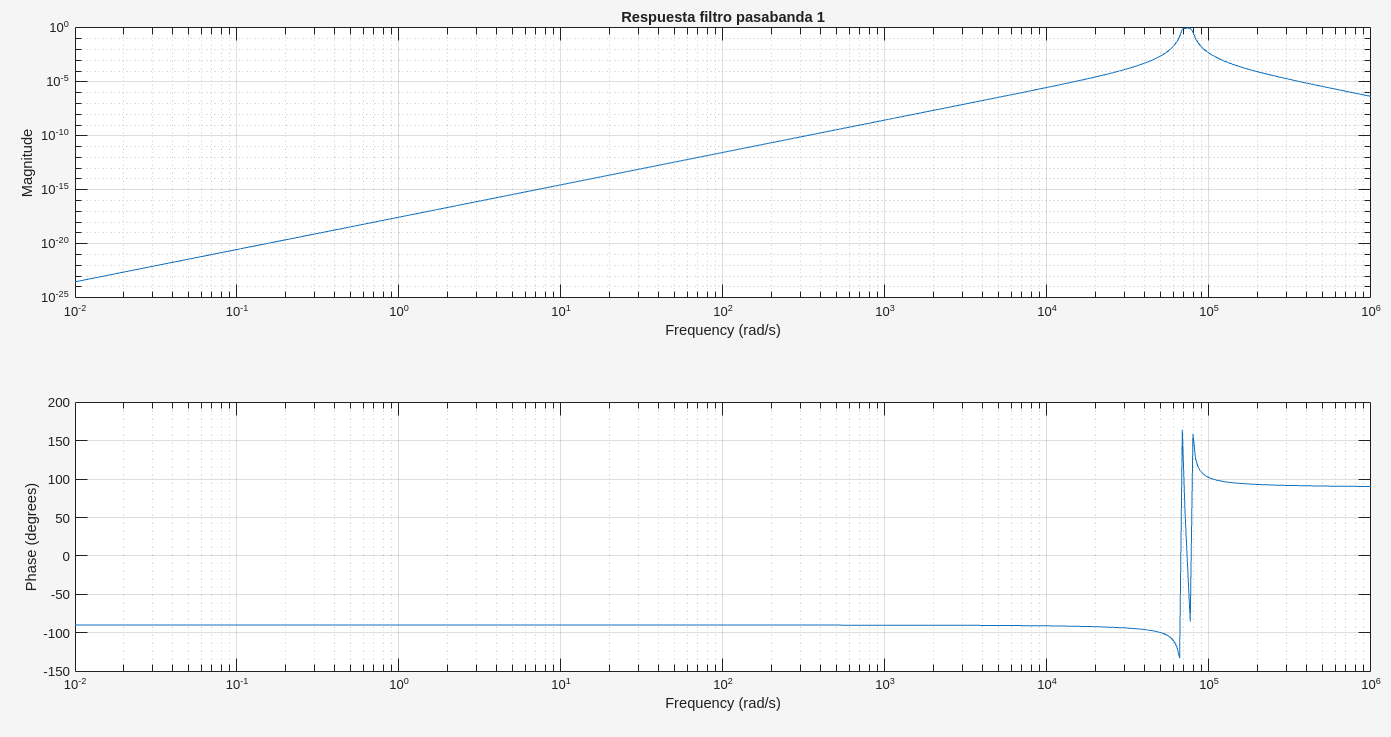
\includegraphics[width=0.42\columnwidth]{figures/Punto1/pasabanda_analogico.png} \\
        \vskip 0.2cm
        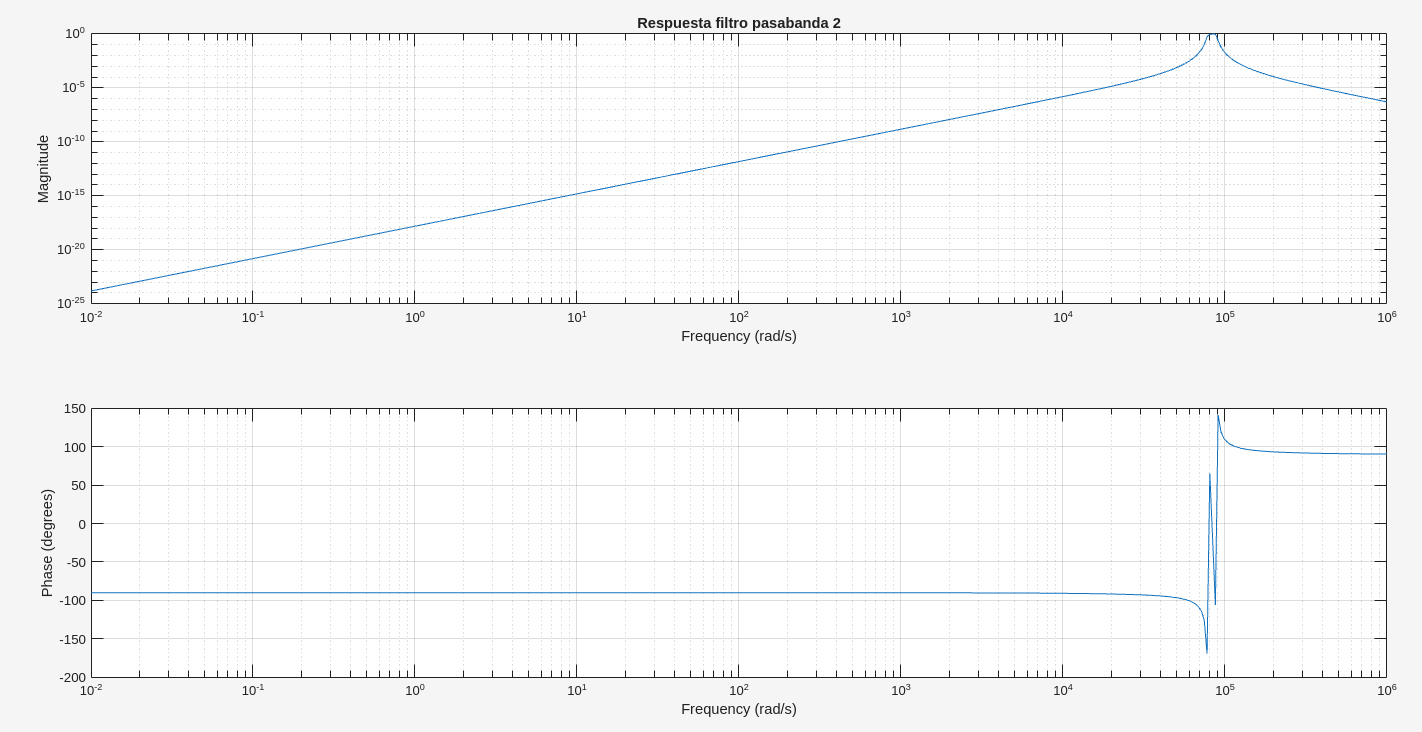
\includegraphics[width=0.42\columnwidth]{figures/Punto1/pasabanda_analogico_2.png}
        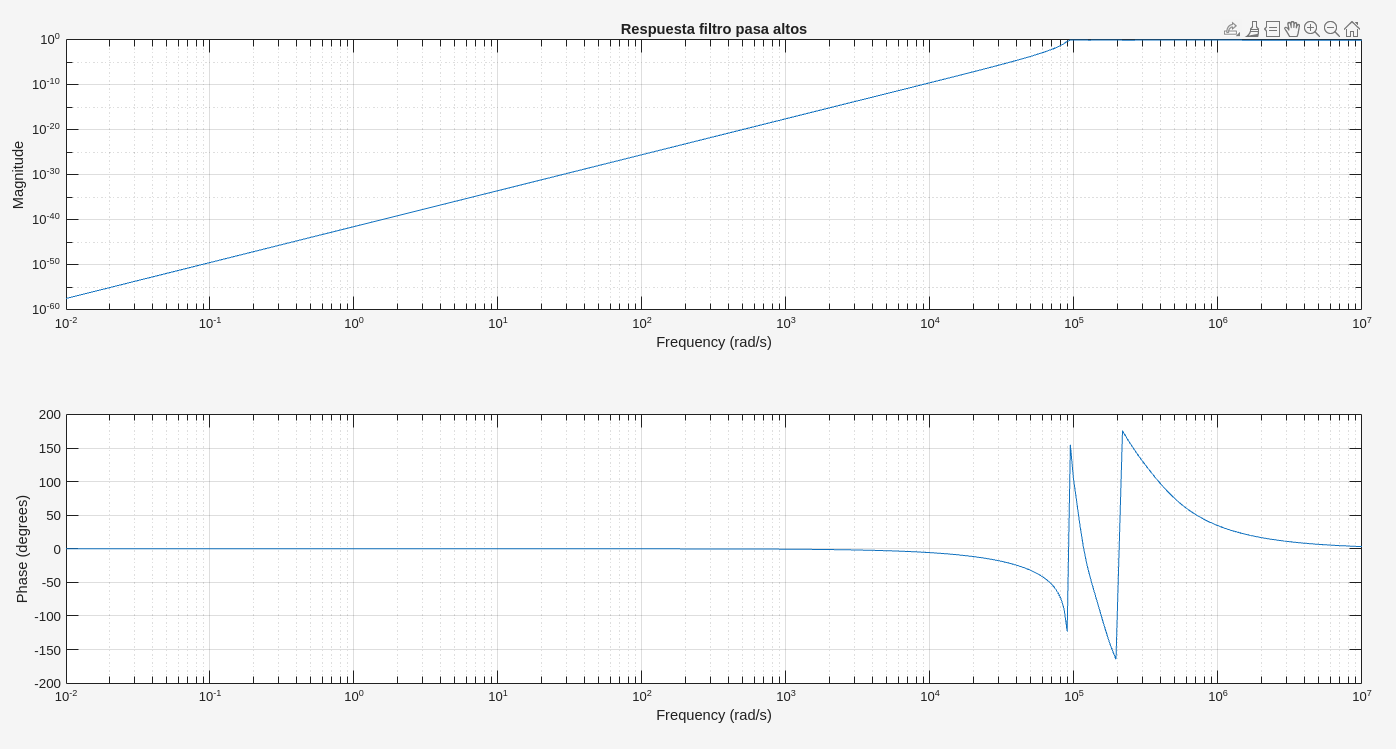
\includegraphics[width=0.42\columnwidth]{figures/Punto1/pasaaltos_analogico.png}
        \caption{Arriba Izq: Filtro pasabajos y Arriba Der: Filtro pasabanda 1. Abajo Izq: Filtro pasabanda 2 y Abajo Der: Filtro pasaaltos.}
        \label{fig:resultados_punto_uno}
    \end{figure}

\section{Punto 2: Diseño de Filtros}

    \subsection{Filtros Analógicos}

        Para la primera iteración de esta etapa, se diseñaron y calcularon los prototipos analógicos basándonos exclusivamente en la familia de filtros de Chebyshev Tipo I. Esta aproximación matemática no fue seleccionada por azar; a diferencia del filtro Butterworth, cuya atenuación es demasiado progresiva para nuestras bandas cercanas, o del filtro de Bessel, que introduce grandes variaciones de fase y ondulación tanto en bandas de paso como de rechazo, el diseño Chebyshev Tipo I concentra un nivel permisible de rizado (\textit{ripple}) paramétrico en la banda pasante pero, a cambio, nos reporta una caída de transición exponencial y escarpada hacia la banda atenuada. Esta selectividad es la piedra angular para lograr delimitar canales con un espaciado de $1.2$ kHz eficientemente y previene que el decodificador confunda frecuencias adyacentes por error. Las frecuencias centrales asignadas a los símbolos son:
        \begin{itemize}
            \item $ f_1 = 10700$ Hz
            \item $ f_2 = 11900$ Hz
            \item $ f_3 = 13100$ Hz
            \item $ f_4 = 14300$ Hz
        \end{itemize}

        La atenuación máxima en la banda de paso permitida fue establecida en $ Rp= 3$ dB, y la atenuación mínima en la banda de rechazo en $W_1 = 15$ dB. Se calcularon las frecuencias de corte como la media geométrica entre las frecuencias de los símbolos. Los órdenes requeridos resultaron en:
        \begin{itemize}
            \item Orden Pasabajos y Pasaaltos: 4
            \item Orden Pasabandas: 2
        \end{itemize}

        A continuación, se presentan las funciones de transferencia obtenidas para cada filtro:

        \textbf{Pasabajos ( $\approx 11.28$ kHz):}
        \begin{equation}
            H_{lp}(s) = \frac{3.166 * 10^{18}}{s^4 + 4.123 * 10^4 s^3 + 5.877 * 10^9 s^2 + 1.443 * 10^{14} s + 4.472 * 10^{18}}
        \end{equation}

        \textbf{Pasabanda 1 ( entre $1.28$ kHz y $2.48$ kHz):}
        \begin{equation}
            H_{bp1}(s) = \frac{2.856 * 10^7 s^2}{s^4 + 4869 s^3 + 1.116 * 10^{10} s^2 + 2.708 * 10^{13} s + 3.094 * 10^{19}}
        \end{equation}

        \textbf{Pasabanda 2 (entre $2.48$ kHz y $3.68$ kHz):}
        \begin{equation}
            H_{bp2}(s) = \frac{2.855 * 10^7 s^2}{s^4 + 4868 s^3 + 1.353 * 10^{10} s^2 + 3.284 * 10^{13} s + 4.551 * 10^{19}}
        \end{equation}

        \textbf{Pasaaltos ( $\approx 13.68$ kHz):}
        \begin{equation}
            H_{hp}(s) = \frac{0.7079 s^4}{s^4 + 1.967 * 10^5 s^3 + 4.885 * 10^{10} s^2 + 2.09 * 10^{15} s + 3.09 * 10^{20}}
        \end{equation}

        La respuesta en frecuencia y los diagramas de polos y ceros corroboran el diseño esperado para las especificaciones analógicas definidas.

        \textbf{Implementación en Secciones de Menor Orden (Punto 5)}
        
        Debido a que el filtro pasabajos sintetizado presenta un orden general de 4, estructurarlo a con hardware como un único circuito con aproximación directa resultaría inestable frente a la tolerancia de los componentes físicos. De acuerdo con los parámetros de la función de transferencia obtenida, la implementación física del filtro analógico debe llevarse a cabo dividiendo $H_{lp}(s)$ en una conexión en \textbf{cascada de dos subsecciones de orden 2} (etapas bicuadráticas). 
        
        Al encontrar las raíces del denominador polinómico original, sus polos complejos conjugados se agrupan en pares para generar dos funciones de transferencia fundamentales del tipo:
        \begin{equation}
            H_i(s) = \frac{k_i}{s^2 + \frac{\omega_i}{Q_i} s + \omega_i^2}
        \end{equation}
        donde $H_{lp}(s) = H_1(s) \cdot H_2(s)$. Esta descomposición modular permite diseñar de forma independiente cada etapa utilizando topologías activas comunes y sólidas de segundo orden, como los circuitos Sallen-Key o la topología de Retroalimentación Múltiple (Multiple-Feedback).

        \begin{figure}[H]
            \centering
            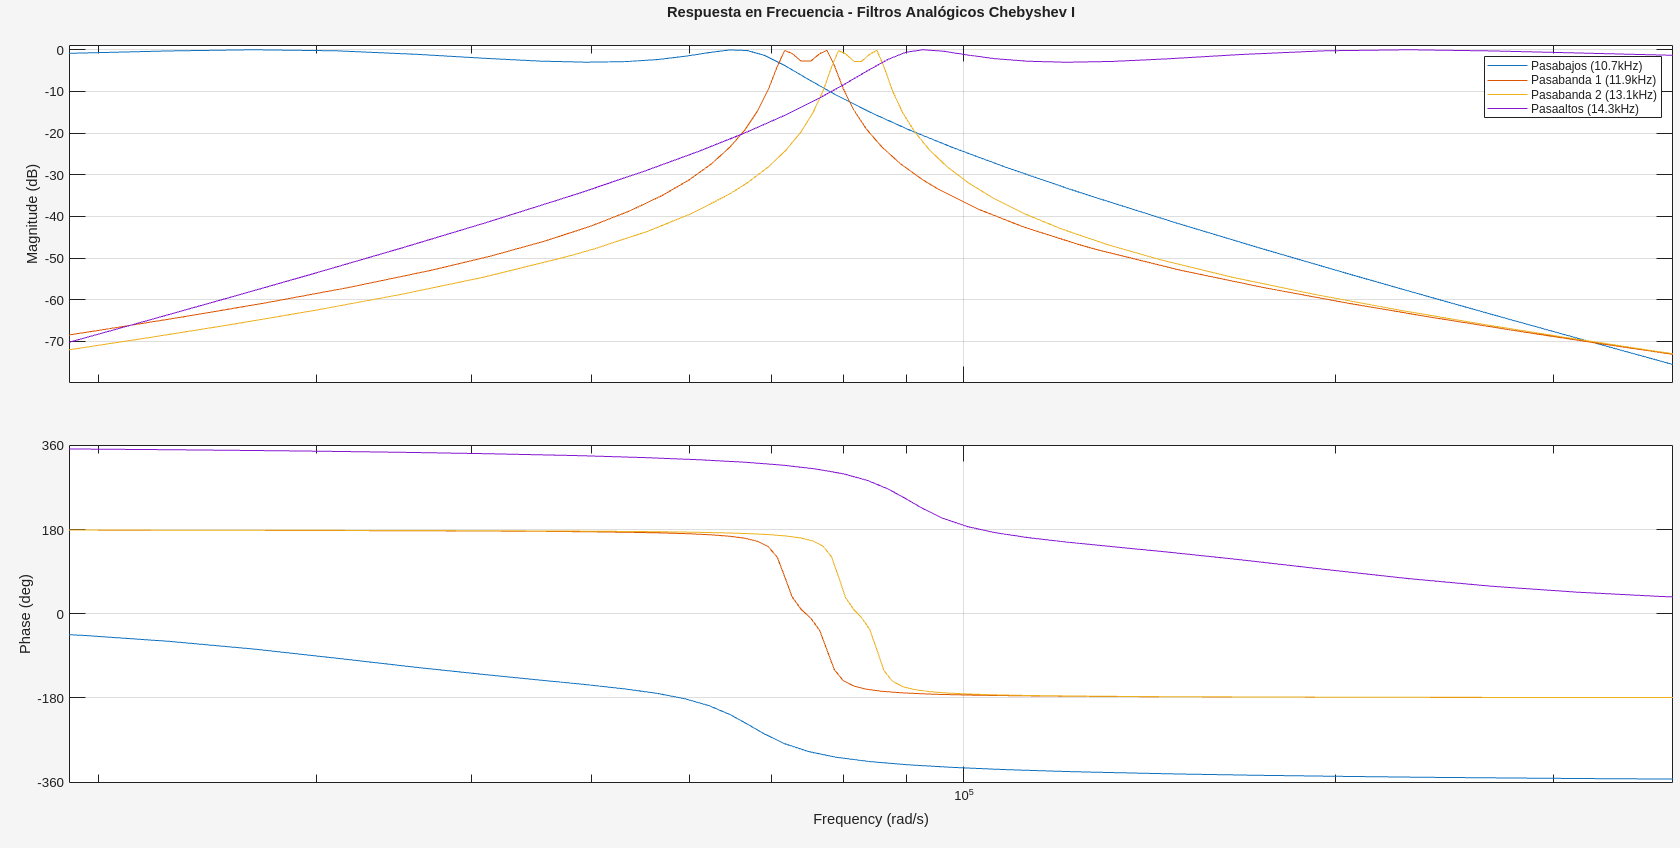
\includegraphics[width=0.75\columnwidth]{figures/Punto2/Bode analogicos.png}
            \caption{Respuesta en frecuencia (Bode) de los filtros analógicos diseñados.}
            \label{fig:bode_analogico}
        \end{figure}

    \subsection{Filtros Digitales (IIR)}

        Para implementar los filtros en un sistema digital que opera a una frecuencia de muestreo de $ f_c= 75$ kHz, se probaron dos técnicas principales: la Transformación Bilineal y la Invarianza del Impulso.

        \textbf{Transformación Bilineal}
        
        La transformación bilineal consta de un procedimiento algebraico de mapeo de planos mediante el cual se proyecta el semiplano izquierdo del dominio $s$ (continuo) directamente en el interior del círculo unitario del dominio $z$ (discreto). Esta sustitución corresponde fundamentalmente a evaluar la integral en tiempo continuo aproximando su área subyacente mediante diferencias trapezoidales (Regla del Trapecio). Su mayor proeza técnica reside en que mapea el eje imaginario entero en una sola revolución dentro del círculo unitario, esquivando de forma radical el solapamiento en frecuencia (Aliasing) inherente a otros métodos. No obstante, por su naturaleza no lineal, esto desata una pequeña deformación asintótica en las frecuencias más altas de la gráfica, fenómeno popularmente conocido como alabeo o \textit{frequency warping}; un problema que mitigamos internamente si se le aplica un cuidadoso factor de pre-warping sobre las frecuencias deseadas. Se usó la función nativa de MATLAB para mapear el dominio $s$ al dominio $z$.

\begin{minted}[linenos,fontsize=\small]{matlab}
[bz_lp, az_lp]     = bilinear(b_lp_a, a_lp_a, Fs);
[bz_bp1, az_bp1]   = bilinear(b_bp1_a, a_bp1_a, Fs);
[bz_bp2, az_bp2]   = bilinear(b_bp2_a, a_bp2_a, Fs);
[bz_hp, az_hp]     = bilinear(b_hp_a, a_hp_a, Fs);
\end{minted}

        \begin{figure}[H]
            \centering
            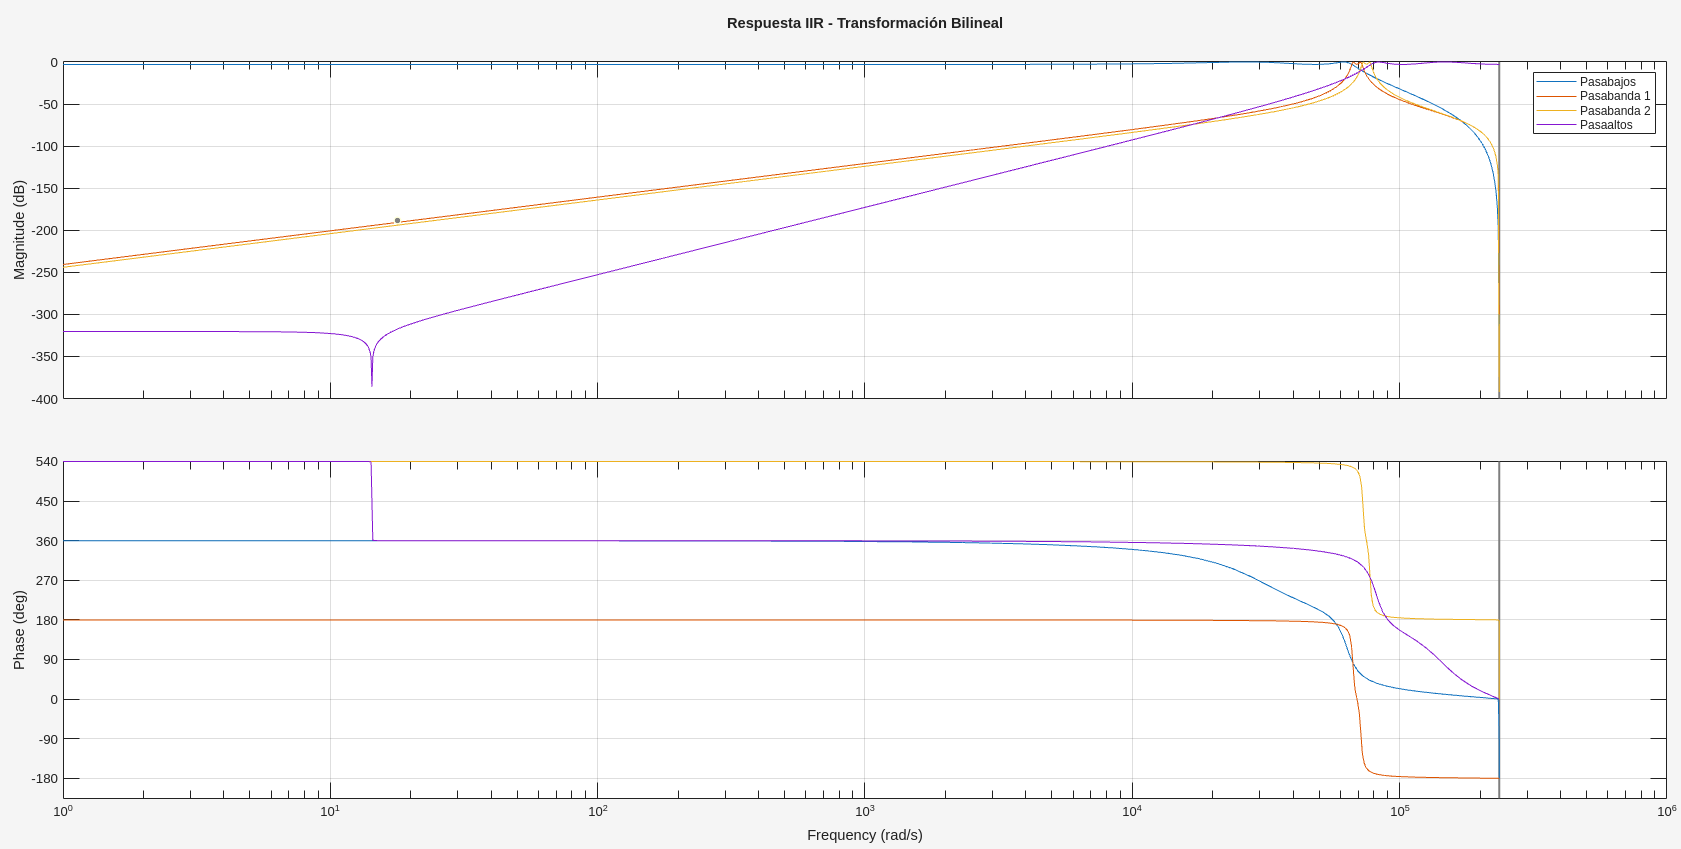
\includegraphics[width=0.75\columnwidth]{figures/Punto2/Bode Digitales.png}
            \caption{Respuesta en frecuencia (Bode) de los filtros digitales con Transformación Bilineal.}
            \label{fig:bode_bilineal}
        \end{figure}

        \textbf{Invarianza del Impulso}
        
        Como método en contraste, se implementó la Invarianza del Impulso, cuya premisa teórica radica en obtener un filtro digital que replique, muestra por muestra de forma calcada, la respuesta al impulso temporal del componente analógico original. Dada su naturaleza puramente muestreada $h(nT)$, adolece de forma flagrante ante la repetición periódica de espectros por el teorema de Nyquist, lo que incurre en aliasing sustancial si la banda a discretizar no se ha confinado de forma estricta a un rango cerrado base. Esto dictamina un postulado empírico clave: este procedimiento resulta inherentemente fallido ante requerimientos Pasaaltos o de Rechaza banda al abarcar infinitas frecuencias en lo continuo. Por ello, dado que la envolvente de la frecuencia $f_4$ nos exigió modelar un componente pasaaltos, nos vimos forzados mediante métodos numéricos o aproximaciones heurísticas a reacomodarlo simulando transitoriamente ser un filtro pasabanda sumamente ancho, para posibilitar medianamente su estabilización convergente durante los cálculos.
        
        \begin{figure}[H]
            \centering
            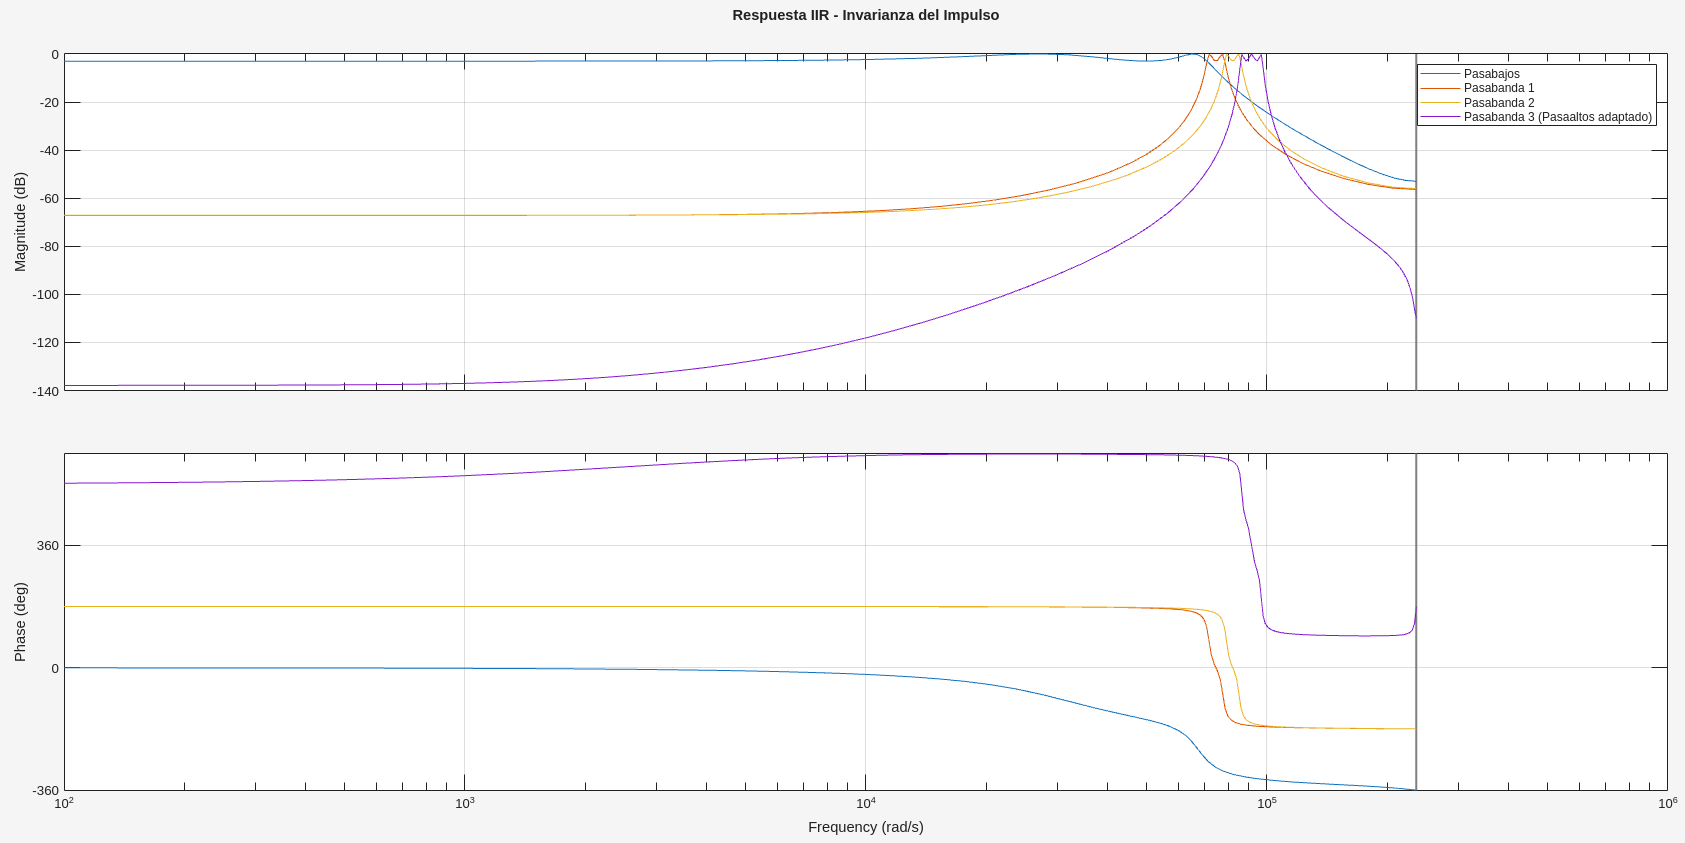
\includegraphics[width=0.75\columnwidth]{figures/Punto2/Bode Digitales Inviarianza.png}
            \caption{Respuesta en frecuencia (Bode) de los filtros digitales con Invarianza del Impulso.}
            \label{fig:bode_invarianza}
        \end{figure}

    \subsection{Elección del Mejor Filtro}
    
    Analizando los métodos, se elige la \textbf{Transformación Bilineal} como el mejor acercamiento para este caso. La principal ventaja de esta transformación es evitar por completo el aliasing. Además, la invarianza del impulso no permite el diseño directo de filtros pasaaltos, lo que obligó a realizar aproximaciones y adaptar el último filtro. Para el demodulador FSK, donde preservar bien la separación frecuencial es crucial para la detección de símbolos, la transformación bilineal otorga un diseño más confiable y exacto en todo el rango requerido, a pesar del posible 'warping' de frecuencia, que en un rango estrecho no presenta impactos severos si se maneja correctamente.

    \textbf{Implementación en Secciones de Menor Orden (Punto 5)}
    
    Al igual que ocurre en el dominio analógico, una implementación directa (\textit{Direct Form}) en software o DSP de un filtro digital de orden alto como este (orden 4) resulta especialmente susceptible a inestabilidades derivadas de la cuantización computacional y al truncamiento finito de sus coeficientes. En la práctica, esto suele traducirse en la desviación perjudicial de sus polos hacia afuera del círculo unitario. 
    
    Por ello, para programar eficazmente el IIR, la rutina principal se divide obligatoriamente en \textbf{secciones de segundo orden en cascada (SOS - Biquads)}. Las fórmulas matriciales en MATLAB, operadas a través de \texttt{tf2sos()}, desglosan el gran polinomio transferencial $H(z)$ en pares de polos y ceros conjugados para conformar la serie:
    \begin{equation}
        H(z) = \prod_{k=1}^{2} \frac{b_{0k} + b_{1k} z^{-1} + b_{2k} z^{-2}}{1 + a_{1k} z^{-1} + a_{2k} z^{-2}}
    \end{equation}
    Garantizando una estructura computacional robusta que previene el desborde aritmético durante la filtración digital.

\section{Punto 3: Diseño de Filtros Digitales (FIR)}

    Debido a que las topologías de Respuesta Infinita (IIR) conllevan obligatoriamente a dependencias retroalimentadas que estiran y distorsionan de forma no-lineal el espectro de fase, consideramos imperativo desarrollar paralelamente un segundo enfoque, construyendo un banco digital de Respuesta al Impulso Finita (FIR). Las grandes virtudes del paradigma FIR se sustentan de forma unánime en que aseguran una configuración inherentemente estable libre de polos inestables (la función solo se proyecta en ceros) y en asegurar una fase calculable estrictamente lineal, lo cual matemáticamente se traduce en ostentar un \textit{retardo de grupo uniforme y constante} en cualquier banda pasante evaluada. Dicho retardo lineal garantiza una fidelidad total de la forma de la onda durante toda su travesía circuital, resultando crucial en flujos de datos y señales moduladas continuas donde las alteraciones asimétricas espurias dictarían un colapso en las lecturas de los decodificadores al disparar la Interferencia Entre Símbolos (ISI).

    La metodología de diseño requerida involucró aplicar la conocida Técnica de Enventanado en Tiempo (\textit{Windowing Technique}). Al truncar simplemente de modo rectangular una respuesta ideal Sinc de alcance infinito, un pernicioso Fenómeno de Gibbs emana fluctuaciones y rizos severos no mitigables en los alrededores de cada corte limítrofe perimetral. En aras de silenciarlas y gobernar la transición, ponderamos los coeficientes empleando explícitamente una \textit{Ventana de Hamming}. La envolvente característica de Hamming modula progresivamente las amplitudes de las muestras laterales bajo un ensanchamiento liso de compana, entregando de este modo un atenuamiento de mitigación formidable sobre el primer y mayor lóbulo lateral (amortiguando ruidos cercanos hasta magnitudes de los robustos y admirables $-43$ dB), demostrando un espléndido equilibrio al conjugar la eliminación en los picos indeseados transitorios simultáneamente con mantener a flote bandas de rechazo de caídas muy profundas.

    Con una frecuencia de muestreo $f_s = 75$ kHz, las frecuencias de corte del Punto 1 (11.3 kHz, 12.5 kHz y 13.7 kHz) se normalizaron respecto a la frecuencia de Nyquist ($37500$ Hz). Luego de probar diferentes aproximaciones analíticas, se estableció un orden estándar $N=200$, el cual aporta la selectividad lo suficientemente abrupta exigida por la cercanía de las bandas del protocolo P25 (separación de 1.2 kHz) para aislar cada canal, dividiendo el espectro en los cuatro filtros requeridos (pasabajos, doble pasabanda, pasaaltos).

\begin{minted}[linenos,fontsize=\small]{matlab}
N = 200;           % orden del filtro
% frecuencias de corte
fc1 = 11300; fc2 = 12500; fc3 = 13700;
% normalización
W1 = fc1/(fs/2); W2 = fc2/(fs/2); W3 = fc3/(fs/2);

% filtro pasabajos
b1 = fir1(N,W1,'low',hamming(N+1));
% filtro pasabanda
b2 = fir1(N,[W1 W2],'bandpass',hamming(N+1));
b3 = fir1(N,[W2 W3],'bandpass',hamming(N+1));
% filtro pasaaltos
b4 = fir1(N,W3,'high',hamming(N+1));
\end{minted}

    \begin{figure}[H]
        \centering
        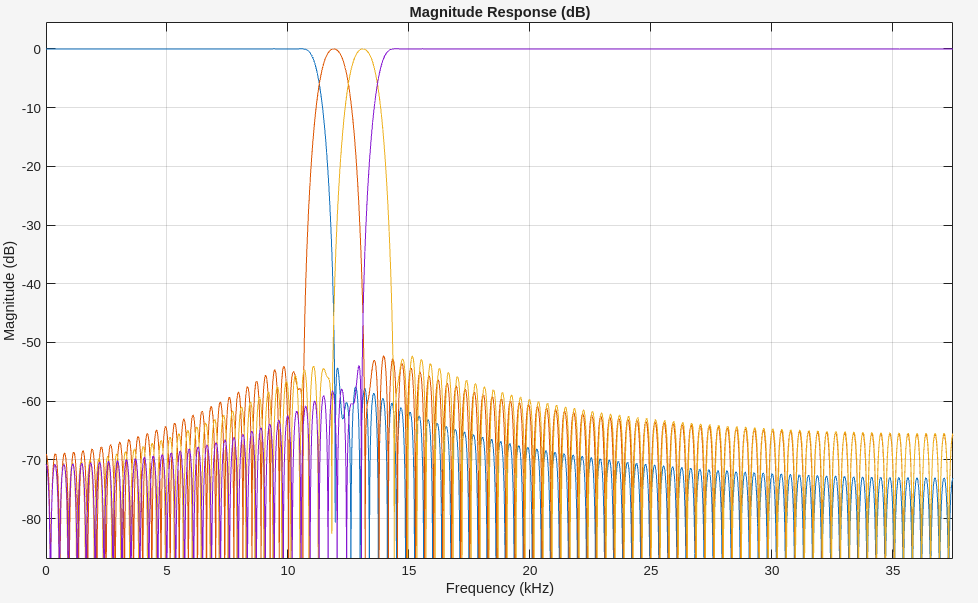
\includegraphics[width=0.75\columnwidth]{figures/Punto3/Filtros_FIR.png}
        \caption{Respuesta combinada en frecuencia del banco de filtros FIR desarrollado.}
        \label{fig:bode_fir}
    \end{figure}

\section{Punto 4: Demodulación y Detección}

    En esta sección se integró a cabalidad el sistema de recepción del esquema FSK, sometiéndolo a las señales de prueba muestreadas y suministradas en la práctica con una frecuencia de $f_s = 75$ kHz (ejemplo evaluativo \texttt{Prueba01} y \texttt{Prueba10}). El banco de filtros actúa separando efectivamente la energía multiplexada de las modulaciones: la información que porta el mensaje atraviesa los umbrales casi inalterada solo a través de uno de los filtros por instante durante su segmento de tiempo único especificado.
    
    El núcleo algorítmico del proceso de detección se culminó al disponer arquitectónicamente y en paralelo un detector de envolvente en el puerto acoplado de salida de cada filtro (computando sistemáticamente la magnitud geométrica de la representación analítica del canal). Esto esencialmente rectifica la señal superior de entrada, desvelando su silueta atenuada global y proyectando directamente su magnitud instantánea. Apoyándonos sobre esquemas superpuestos comparadores temporizados, se evaluó en sincronía qué enrutamiento presentó la cresta de dominancia modal (máxima amplitud) de todo el conjunto al mismo tiempo. Al aislar esa mayoría comparativa, se dictamina certeramente cuál frecuencia dominante poseía el transmisor, y de allí se extrapola, de manera codificada preacordada, cómo esa portadora resuelta corresponde bit a bit hacia el símbolo equivalente exigido por el protocolo P25 ($+3, +1, -1, -3$).
    
    El simulador central concedió comprobar íntegramente cómo las tres topologías (Analógica, IIR vía Integración Bilineal y paradigma paramétrico FIR) logran de manera cabal su función fundamental y discriminatoria FSK. A la postre y como corolario vital para implementaciones duras: mientras un IIR de bajo orden induce un sutil entorpecimiento temporal no lineal oscilatorio "ringing" que distorsiona las fronteras por sus desfases relativos, la estructura FIR (disipadora de alinealidad a cambio de altos recursos de computación u órdenes superlativos de $N$) dictaminó en nuestra simulación poseer la rectitud más nítida concebible confirmando que sigue representando la élite como patrón de trabajo y la vía más pragmática del procesamiento en sistemas a gran escala como DSPs y redes modulares rápidas.
    
\begin{minted}[linenos,fontsize=\small]{matlab}
% Filtrado de la señal FIR elegido
y1 = filter(b_fir_lp, 1, x);
y2 = filter(b_fir_bp1, 1, x);
y3 = filter(b_fir_bp2, 1, x);
y4 = filter(b_fir_hp, 1, x);
\end{minted}
    
    \begin{figure}[H]
        \centering
        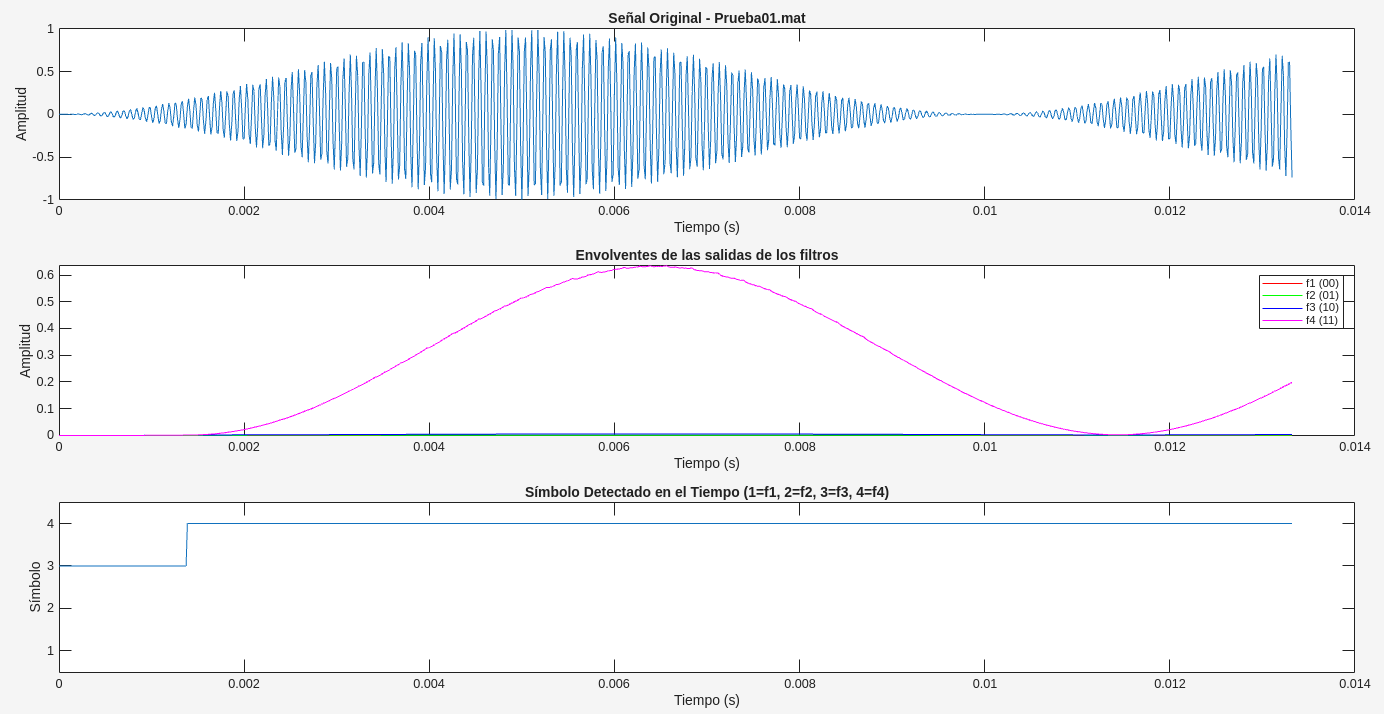
\includegraphics[width=0.75\columnwidth]{figures/Punto4/Prueba01_FIR.png}
        \caption{Demodulación de envolventes tras el banco de filtros FIR para el conjunto de prueba Prueba01.}
        \label{fig:prueba_01_fir}
    \end{figure}

\section{Demodulación de la señal FSK}

Una vez diseñado el banco de filtros, se procede a la demodulación de la
señal FSK. El objetivo es identificar, para cada intervalo de tiempo,
cuál de las frecuencias está presente y así recuperar la secuencia de
bits transmitida.

\subsection{Segmentación de la señal}

La señal recibida se divide en segmentos de duración igual al símbolo.
Dado que la duración del símbolo es

\begin{equation}
T_s = 10\;ms
\end{equation}

y la frecuencia de muestreo es

\begin{equation}
f_s = 75\;kHz
\end{equation}

el número de muestras por símbolo es

\begin{equation}
N = f_s \cdot T_s = 750
\end{equation}

Cada segmento de 750 muestras corresponde a un símbolo.

\subsection{Filtrado mediante banco de filtros}

Cada segmento de la señal es procesado a través del banco de filtros FIR
diseñado previamente (pasabajos, dos pasabanda y pasaaltos). De esta
forma se obtiene una salida por cada filtro, correspondiente a cada una
de las posibles frecuencias del sistema FSK.

\subsection{Cálculo de energía}

Para determinar cuál frecuencia está presente en cada símbolo, se calcula
la energía de la señal a la salida de cada filtro:

\begin{equation}
E_k = \sum_{n=0}^{N-1} |y_k[n]|^2
\end{equation}

donde $y_k[n]$ corresponde a la salida del $k$-ésimo filtro.

La frecuencia detectada será aquella cuya energía sea máxima:

\begin{equation}
k = \arg\max(E_1, E_2, E_3, E_4)
\end{equation}

\subsection{Asignación de bits}

Cada frecuencia detectada se asocia a un par de bits de acuerdo con la
codificación del sistema:

\begin{center}
\begin{tabular}{|c|c|}
\hline
Frecuencia & Bits \\
\hline
$f_1$ & 11 \\
$f_2$ & 10 \\
$f_3$ & 00 \\
$f_4$ & 01 \\
\hline
\end{tabular}
\end{center}

De esta manera, cada símbolo produce dos bits.

\subsection{Reconstrucción del mensaje}

La secuencia de bits obtenida se agrupa en bloques de 8 bits, los cuales
se interpretan como caracteres ASCII.

\begin{equation}
\text{Carácter} = \text{ASCII}(\text{bits})
\end{equation}

Este proceso permite reconstruir el mensaje transmitido a partir de la
señal FSK.

\subsection{Implementación en MATLAB}

El proceso completo se implementa mediante el siguiente código:

\begin{verbatim}{matlab}
Ns = length(x)/750;
bits_total = [];

for k = 1:Ns
    
    inicio = (k-1)*750 + 1;
    fin = k*750;

    segmento = x(inicio:fin);

    y1 = filter(b1,1,segmento);
    y2 = filter(b2,1,segmento);
    y3 = filter(b3,1,segmento);
    y4 = filter(b4,1,segmento);

    E = [sum(y1.^2) sum(y2.^2) sum(y3.^2) sum(y4.^2)];

    [~,idx] = max(E);

    if idx == 1
        bits = [1 1];
    elseif idx == 2
        bits = [1 0];
    elseif idx == 3
        bits = [0 0];
    else
        bits = [0 1];
    end

    bits_total = [bits_total bits];
end

% Conversión a ASCII
mensaje = '';

for k = 1:8:length(bits_total)
    byte = bits_total(k:k+7);
    num = bin2dec(num2str(byte));
    mensaje = [mensaje char(num)];
end

disp(mensaje)
\end{verbatim}

\subsection{Resultados esperados}

Al aplicar el procedimiento descrito, se obtiene como salida el mensaje
original transmitido, demostrando así la correcta operación del sistema de
demodulación FSK basado en un banco de filtros FIR.

\end{document}